\documentclass[tikz,border=4pt]{standalone}
\usepackage[utf8]{inputenc}
\usepackage[T1]{fontenc}
\usepackage{amsmath}
\usepackage{pgfplots}
\usepgfplotslibrary{groupplots}
\pgfplotsset{compat=1.18}
\begin{document}
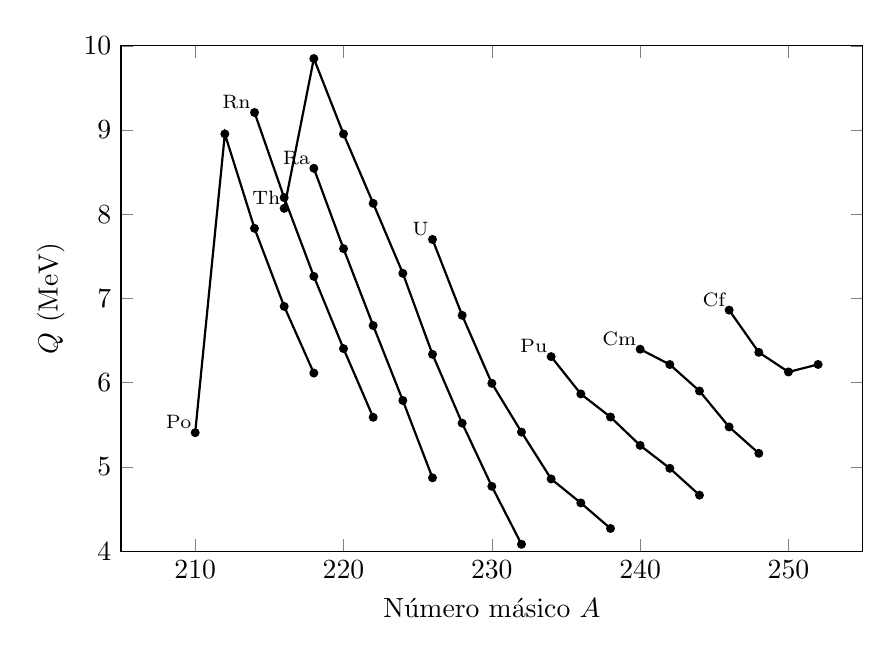
\begin{tikzpicture}
\begin{axis}[width=11cm, height=8cm, xmin=205, xmax=255, ymin=4, ymax=10,
  xtick={210,220,...,250}, ytick={4,5,...,10},
  xlabel={N\'umero m\'asico $A$}, ylabel={$Q$ (MeV)}, clip=false]
\addplot[thick, mark=*, mark size=1.2pt] coordinates {(210,5.407) (212,8.954) (214,7.833) (216,6.906) (218,6.115)} node[pos=0,above left,font=\scriptsize,inner sep=1pt]{Po};
\addplot[thick, mark=*, mark size=1.2pt] coordinates {(214,9.208) (216,8.198) (218,7.263) (220,6.405) (222,5.59)} node[pos=0,above left,font=\scriptsize,inner sep=1pt]{Rn};
\addplot[thick, mark=*, mark size=1.2pt] coordinates {(218,8.546) (220,7.592) (222,6.679) (224,5.789) (226,4.871)} node[pos=0,above left,font=\scriptsize,inner sep=1pt]{Ra};
\addplot[thick, mark=*, mark size=1.2pt] coordinates {(216,8.07) (218,9.849) (220,8.953) (222,8.13) (224,7.299) (226,6.337) (228,5.52) (230,4.77) (232,4.082)} node[pos=0,above left,font=\scriptsize,inner sep=1pt]{Th};
\addplot[thick, mark=*, mark size=1.2pt] coordinates {(226,7.701) (228,6.8) (230,5.993) (232,5.414) (234,4.858) (236,4.573) (238,4.27)} node[pos=0,above left,font=\scriptsize,inner sep=1pt]{U};
\addplot[thick, mark=*, mark size=1.2pt] coordinates {(234,6.31) (236,5.867) (238,5.593) (240,5.256) (242,4.984) (244,4.666)} node[pos=0,above left,font=\scriptsize,inner sep=1pt]{Pu};
\addplot[thick, mark=*, mark size=1.2pt] coordinates {(240,6.398) (242,6.216) (244,5.902) (246,5.475) (248,5.162)} node[pos=0,above left,font=\scriptsize,inner sep=1pt]{Cm};
\addplot[thick, mark=*, mark size=1.2pt] coordinates {(246,6.862) (248,6.361) (250,6.128) (252,6.217)} node[pos=0,above left,font=\scriptsize,inner sep=1pt]{Cf};

\end{axis}
\end{tikzpicture}
\end{document}
